\documentclass[format=acmsmall, review=false, screen=true]{acmart}
\settopmatter{printacmref=false} % Removes citation information below abstract
\renewcommand\footnotetextcopyrightpermission[1]{} % removes footnote with conference information in first column
\pagestyle{plain} % removes running headers
\acmYear{2017}
\acmMonth{12}

\usepackage[utf8]{inputenc}
\usepackage{microtype}
\usepackage{amsmath}
\usepackage{listings}
\usepackage{amsmath}
\usepackage{float}
\usepackage{wrapfig}
\usepackage{subcaption}
\usepackage{dirtytalk}

\lstset{
  basicstyle=\ttfamily,
  columns=fullflexible,
  frame=single,
  breaklines=true,
  postbreak=\mbox{\textcolor{red}{$\hookrightarrow$}\space},
  aboveskip=10pt,
  belowskip=5pt,
  tabsize=2
} 

\setlength{\textfloatsep}{14pt}
\setlength{\abovecaptionskip}{4pt}
\setlength{\belowcaptionskip}{4pt}

\author{Richard Bányi}
\author{Israe Noureldin}
\author{Islam Jabrayil Mastanov}
\author{Soltan Reza Hoseini}
\author{Thomas Roberts}

\title{\textsc{Project One} - Data Detox}
\acmDOI{}
\begin{document}
\maketitle 

\section{Introduction}
In contemporary society, where the internet has transformed the foundation of business and economics, telecommunication, transportation and basically every other major industry, data becomes one of the products of such transformations. Therefore the technologies around Big Data are a vital element of this network infrastructure.

For that reason, there has been a massive attention towards the protocols in which the Internet is facilitated, and towards the different technologies around data storage, data mining processes, data analytics, developing algorithms and machine learning, social media and so on. As we enthusiastically move into the future and embrace different digital tools and technologies such as smartphones, smart TVs, Chromebooks, and Ultrabooks, we learn that there is little notice among the general population regarding data privacy and data protection, especially when one might learn about the amount of data being produced from people’s activities across different social media channels and platforms such as Facebook, Instagram, Snapchat etc.

This paper is a brief report and a group-reflection upon practices surrounding the awareness of data privacy, data ownership and power struggles in the age of the Internet. It will also cover individuals’ rights to control their own data and accept social responsibility for their data practices.


\section{Discussion}
Before starting this section, we believe it is important to mention that instead of using our notes from Data Detox week, we decided to use our notes from the Data Detox discussion. We spent half a day discussing and comparing our experiences throughout the Data Detox week and that has lead us to some interesting points and questions.
 
With the Internet deeply rooted in the foundational layers of society and economics, it is almost impossible to imagine a world without internet, especially when this technology has become so effective at improving our lives in many ways such as knowledge and information sharing, health care, education, environment etc.
During our Data Detox discussions, we have come up with two major approaches when we discussed power struggle in the age of Internet and data ownership, data accessibility and accountability.
 
Two approaches:
\begin{itemize}
		\item\say{Some giant companies such as Facebook, Amazon, and Google dominate the advertising market and cloud data storage, and that results in some corporations becoming very powerful, which raises concerns about the future of the Internet} [quote Soltan]. 
		\item\say{In contemporary society, in every field and industry, there are a number of powerful players, and if Google gets so powerful, it doesn’t affect me as long as I know they are not using their power in the wrong way} [quote Israe].
\end{itemize}

Both approaches deserve further discussion because both open new approaches and concerns towards the future of the Internet. One simple and obvious question that came up was why these companies are collecting so much information. Well it’s deeply rooted in their business model.
As Shoshana Zuboff popularizes, we live in an age of Surveillance Capitalism. She states that \say{the online world, which used to be kind of our world, is now where capitalism is developing in new ways.} Moreover Nick Couldry believes that \say{surveillance capitalism is focused on data extraction rather than the production of new goods, thus generating intense concentrations of power over extraction and threatening core values such as freedom and privacy.}
The primary goal of social platforms, the advertisement industry, and all other digital products/services is to keep capturing our attention, to persuade us to behave in a certain way, to buy one more pair of shoes in the context of profit making. By capturing our usage of their services, it allows them to survey and shape opinions with machine learning at scale. These methods can determine our identities and moods. With all of this power, it is a perfect set up for totalitarianism. However, we would argue that Silicon Valley companies are still kind of liberal if we compare them to other large players such as China. The key observation is that all of the influence exerted by such players is happening in the dark, behind the scenes, and moreover it is targeted at individuals rather than at a group in open space. On TV, companies advertise to everyone, but on the internet it’s fragmented and profiled. We don’t see what other people are seeing. This gives the power to companies to figure out what people are up to.
This might present a danger. Certain organizations might take advantage of it and misuse it for their own selfish intentions. An example for this could be seen in the recent American elections when the Russian government allegedly misused Google/Facebook algorithms to disseminate fake news and potentially managed to manipulate/persuade voters. Therefore we think the key point is the realization of the manipulative intentions of these services.
However, we think persuasion is just persuasion. It may not be a problem. There are times when we’re fine with what captures our attention. We have to understand the dangers that algorithms can impose and have to make our own decisions. Whatever power we grant to these companies, we have to understand what the consequences can be and how and when companies should have access to our private information.
 
Another commonality that came up was about the \textit{right to be forgotten}. Several of us had produced data on Facebook and Instagram in the past that at the time we felt was important enough to share. Having matured and having changed opinions since then, it was no longer important to us, and we wanted to remove it. It was possible to go through posts, photos etc. one-by-one and remove them, but this was tedious and time-consuming. We used a chrome extension called Data Selfie which gave us a really good overview of what Facebook knows about us. Unsurprisingly, the Facebook algorithms were able to gain lot of insights about us, for example religious and political orientation, shopping, health and other preferences. What surprised us the most is the fact that Facebook even stores data that we did not publish. \say{We were able to see the data that we have input in the post or comment field without submitting} [quote Richard]. Similarly, if we wanted to change or delete a social media profile, we found that \say{search engines like Google had cached versions of these old profiles that were still being included in the results} [quote Tom]. This led us to reflect on how the data that is important to us now may not be important to us in 10 years’ time. This suggests that the set of data we consider important is not fixed and is in fact always changing, and the right to edit or delete data is imperative. Furthermore, even when we are given the option to delete and edit our data, this may not impact any analyses that companies have already performed and stored. In this regard, we may be able to freely edit our \textit{visible} data but we actually have limited access to, and control of, our \textit{inferred} data.
Another topic we have discussed was deleted data: when one’s data is deleted, is it deleted from the internet? If one deletes a picture or a tweet from their account, is it deleted from the databases? How can the deleted data affect the profiling issues we are facing? Digital services we use today are often not designed by default to give the option to users to delete their data, and permission is not given to users to completely wipe out their history of digital interactions.
This can hint at the opinion of Richard Stallman on using digital services, as he puts it: \say{If you use a proprietary program or somebody else's web server, you're defenseless. You're putty in the hands of whoever developed that software.}
Interestingly, multiple members of our group created and started using a Facebook profile once enrolling at university as it was the best means of communication with other students. This is another example of how it is almost impossible to participate socially in society where these platforms have become the status quo. Although members had different reasons for not using Facebook prior to starting the university, one of our members specifically avoided its use due to his concern over Facebook's proprietary use of data. say{Going through the Data Detox and being familiar with most of the tools and techniques provided, it was surprising for me to see the limited use of them among my constituents who were not aware of the privacy violations they are subjected to.} [quote Islam]. Elaborating on this as a group has led us to presume how much of the world's population may be completely unaware about the data being collected on them.


\section{Data-fasting and Opting-out are not a solution}

With the internet rooted so deeply in developed countries’ infrastructure, it is impossible to stop using digital services, as Janet Vertesi experienced when trying to keep her pregnancy a secret made her confront her family members and friends and even a suspicious member of the society. Google and Facebook dominate the digital market and by going online and using digital services, in one way or another, we interact with these companies. In particular, using LightBeam in day 6 of Data Detox showed how Google and Facebook know where you are and how you are interacting with other digital services, even when the user is not interacting directly with them.

\begin{figure}[H]
  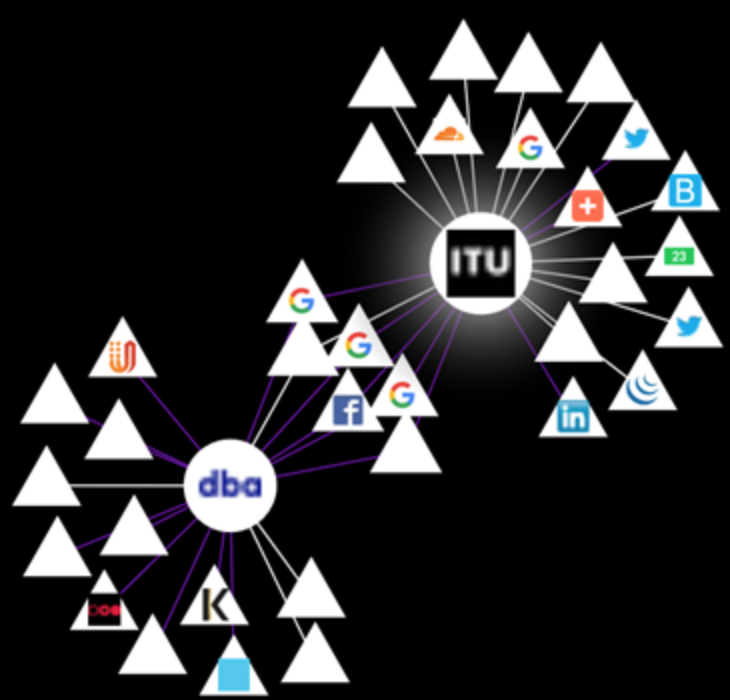
\includegraphics[width=0.46\linewidth]{lighbeam.PNG}
  \caption{Visualisation using LightBeam showing the 3rd party websites (triangle nodes) that your browser connects to when a user directly connects to 2 websites (circle nodes: ITU.dk, DBA.dk).}
  \label{fig:main-diagram}
\end{figure}

During the data-fasting session, we also experienced that it will become a pain if we stop producing data. This hints towards how important it can be to seek out solutions to protect personal data, especially in an era where there is more focus on advancing technology than discussing what privacy is and how to protect it.

In the recent turmoil surrounding Edward Snowden’s leaks against the NSA, we know that the NSA has access to information stored by major IT companies in the US. Relating this to the quote by Stallman, we become putty in the hands of free-service providers. As Google, Amazon and Facebook become more rich and powerful (either by growth in their business or by buying other giant IT companies), operating and existing on the internet poses a higher risk of leaving traces and giving away data to these large tech companies. Considering that even when we don’t use services provided by Google and Facebook, they still know what we are, where we are and what our interests are, it can hint at a world where everything is controlled by a few players, and their monopoly can add fuel to the surveillance capitalism theory or approach. Google is trying to provide internet to one billion people who don’t have access to the internet. Facebook buys Whatsapp and tries to buy Snapchat or pushes it out of the market by fierce competition against them. These examples show that this digital world is increasingly becoming about power, control and money, a world where individuals become a source to feed these giant engines of power. It is perhaps a step too far to imagine a world described by George Orwell in 1984, but it is naive to think that such a future is absolutely impossible. When one entity or individual grows an interest in acquiring more control, it is not too far to think that they may soon acquire more power. In the case of Amazon, Facebook and Google, this control of the internet is getting bigger to the extent that they could have interests in policy making in different countries and being involved in politics. Having considered the NSA story, and digital surveillance, this growth can hint at a dangerous future for the internet and virtual world, which used to be a representation of freedom 10-15 years ago. So it is important more than ever to remain engaged, and to be aware of this power struggle, to analyze and talk about this issue and educate people around us, because if one thing can stop this, it is the power that lies within a network or group of people. [quote Soltan]

\section{Databox}
The goals of the Databox (Haddadi 2015) are interesting as it tries to find a compromise between the \textit{all or nothing} situation users often find themselves in nowadays: either they forfeit their privacy to use a service, or they are not able to use services that are often deeply ingrained in society. It aims to give attractive incentives to both the companies wishing to use people's data, and the data subjects themselves to find a compromise in data privacy. The ideas put forth have the potential to find this middle ground: those who want to continue to use services as they are today can \textit{pay with their privacy}, whilst others can protect their privacy and pay for the services using money. This could allow more privacy-conscious users to remain private while still being able to use modern, networked services.

It’s clear that there are still some major technical hurdles to overcome, and the paper’s section on \textit{complexity} notes that previous attempts at similar concepts have had differing levels of success. For instance, storing all of a person’s data in one place inherently makes it a \textit{honey pot} that is attractive for an adversary to attack. Therefore, security and availability is critical and managing this single point of failure is a major problem to solve. Such issues bear resemblance to those faced by Password Management services such as LastPass and 1Password. LastPass has been subject to several breaches in recent years but a combination of strong security measures, dedicated response teams, and clear communication with its users has ensured that the private data entrusted to them remains secure. Similarly, in the fallout of the \textit{Global Surveillance Disclosures} (2013-present) of Edward Snowden, 1Password has faced questions from its users (Goldberg, 2013) about how they operate a secure system in a world where government entities may attempt to undermine it.

One could argue that for many people, passwords are perhaps the most sensitive piece of private data they have, and we feel that if Databox implements its architecture akin to password management systems, it will have the highest chance of success from a technical perspective. More concretely, it should use strong hashing and encryption techniques to obfuscate data so that even in the event of a security breach, it is difficult to get any value from the stolen information.

In the section on availability, the Databox authors favour pushing its storage to the cloud using Internet-based servers. While this indeed will help with availability, they acknowledge that it may come at the cost of trust. We once again draw parallels with password managers whereby many only encrypt and store data locally on the user’s machine by default, and activating their browser or cloud-based service is optional (in an effort to minimise the number of parties that ever touch the data). Therefore, we feel that encrypted data should ideally be stored locally on the data subject’s machine rather than in the cloud, and any cloud-based storage of encrypted data should use end-to-end encryption so that even Databox (or any IaaS provider it uses, like Amazon or Google) cannot intercept the communication and view unencrypted data.
Something that Databox should be very aware of is how they design the systems that users will use to interact with their Databox. As Goldberg writes in his blog post, \say{Only communications tools appear to be targeted… [Adversaries] would rather go around 1Password than through it.} Similarly, some of the LastPass breaches have targeted its web browser plugins for Firefox and Chrome to launch phishing attacks rather than targeting the LastPass system itself, mainly because web browsers provide a much wider surface of attack.

Closely related to this point, it is interesting that a key point of Databox is its usability. It is next to useless to provide the level of control on offer if an ordinary user is not able to understand exactly what their data says about them, and what third-party services can infer about them. We question whether the average user has the capabilities and knowledge to act properly when given this power (without guidance), for example, knowing how to recover after a data breach. Moreover, we discussed how having the power to edit and delete the entirety of our data could exacerbate the \textit{perfect record} issue often debated in social media settings.
We also think that giving this power directly to users could be beneficial psychologically as subjects feel empowered that they have fine-grained control over what is known about them, and how this knowledge is used. This could shift the notion of consent away from simply agreeing to hand data over, and instead move towards agreeing to having certain conclusions drawn about you. However, to even reach this point, collecting and merging data from the plethora of existing (and often proprietary) sources in the first place is a difficult task. Keeping this information updated and synchronised across devices also adds to the complexity.

Even if the technical infrastructure is in place, it is not clear how early adopters will be encouraged to get onboard with Databox. A service such as this would only truly work according to the \textit{network effect} where it is only attractive if it already has people and companies using it.

The main question one might ask is that how Databox can help to protect one’s data against the giant data corporations. For that reason, we don’t assume that Databox can make a user in charge of their data that are owned by Twitter, Facebook, Google or Apple. The paper highlights how a key benefit for third parties that want to access data is that even if this proprietary data is still stored in \say{centralised silos} by large companies, Databox could use APIs and offer a way to merge and integrate all of these sources into one place. We found this insight quite striking and disturbing as we envisage how this could give the potential for a whole new level of inferences to be drawn about people. From a technical standpoint, Databox could almost act like a Data Warehouse that draws information from various sources and organises it in a way that is easy to query. Although there is already some degree of data sharing between companies, data is typically proprietary and analyses are performed \textit{within} data silos. It is foreseeable that if the project is successful, a company could (with user consent, of course) draw conclusions across all of these silos and make even stronger conclusions about people than has ever been possible.

In the paper \say{A critical review of 10 years of Privacy Technology}, Danezis and Gurses describe privacy as confidentiality: \say{privacy is hence defined as avoiding making personal information accessible to a greater public. If the personal data becomes public, privacy is lost.} Moreover privacy is described as control: \say{the right of the individual to decide what information about himself should be communicated to others and under what circumstances.}

If we apply the lens of privacy as confidentiality to Databox, it technically provides privacy to individuals because users decide whom to share their data with and for how long, it keeps users in control of their data even when they have granted access to a company, they still have the option to stop this access.

If we look at the technology through the second lens which is privacy as control, this is still a good solution to choose what information should be communicated to whom and under which circumstances. However, as we discussed earlier, we still haven’t understood how Databox can challenge the fact that giant companies have access to and store users’ data. In short, this technology can provide grounds to have control over your data against smaller companies, but not so much against big companies where we pay for the services with our data, so in that sense it can only be a partial solution.

An important concept of the Databox seems to be to provide a way to decentralise how data is stored. If \textit{data silo} companies continue to store private data and decide how it is accessed and used, any conflicts of interest these companies have with third parties could have implications on the users whose data they are storing. Providing a decentralised option could take away this control and limit negative effects in this regard.

\section{Conclusion}
Technologies such as Databox, regulations such as GDPR, and practices such as opting out of the digital world are not the ultimate solutions, but these partial solutions are needed to engage the general population, to encourage innovators to focus on this issue and build upon them. They are essential to move forward, to appropriate further innovation and lay the foundations of a future where people are more aware and capable of protecting their privacy and personal data.

We need to move towards a future where digital services are by design meant to give privacy and protection to individuals, a future where the answer to privacy is not Databox or opting out.

It is true that each individual needs to accept and be aware of their digital behaviour and be accountable for what they do, and be aware of the consequences of paying for digital services they use with their data. On the other hand, service providers by design limit the amount of control each user has over their data, so the questions remain to be: how much control over our digital presence we acquire even if we accept the responsibilities that come with using digital service? Should one stop using Internet services completely? What happens when individuals are forced to use digital services to interact with government to, for example, fix their taxes or to use social and health services? Where is the line between accepting responsibility and taking control drawn?

To summarize, we conclude by emphasizing that this topic is so broad and at the same time can be so cloudy and vague that it takes time and effort to solidify these concepts and draw the lines between different concepts and definitions such as privacy, data protection or taking control of personal data. This topic needs more attention, more discussion and innovation, and hopefully with these engagements, we can see a better and more private future for each individual in the Internet era.
\newpage
\begin{thebibliography}{9}
\bibitem{couldry} 
Couldry, N. (2014). The price of connection: ‘surveillance capitalism’.
\\\texttt{https://theconversation.com/the-price-of-connection-surveillance-capitalism-64124}
 
\bibitem{danezis} 
Danezis, G. {\&} Gürses, S. (2010). A critical review of 10 years of privacy technology. Proceedings of surveillance cultures: a global surveillance society, 1-16

 
\bibitem{stallman} 
Stallman, R. (2008). Cloud computing is a trap, warns GNU founder Richard Stallman\\\texttt{https://www.theguardian.com/technology/2008/sep/29/cloud.computing.richard.stallman}

\bibitem{vertesi} 
Vertesi, J. (2014). My Experiment Opting Out of Big Data Made Me Look Like a Criminal.
\\\texttt{http://time.com/83200/privacy-internet-big-data-opt-out/}

\bibitem{zuboff} 
Zuboff, S. (2014). Reality is the Next Big Thing: Keynote.
\\\texttt{http://davidcharles.info/2015/01/shoshana-zuboff-surveillance-capitalism/}

\bibitem{datax} 
DATA X. Data Selfie.
\\\texttt{http://www.dataselfie.it/}

\bibitem{haddadi} 
Haddadi, H. (2015). Personal data: thinking inside the box

\bibitem{goldberg} 
Goldberg, J. (2013). Password and The Crypto Wars. \\\texttt{https://blog.agilebits.com/2013/09/06/1password-and-the-crypto-wars/}

\end{thebibliography}

\end{document}
